\chapter{Literature survey}

\section{Introduction}
This chapter covers the literature in the field of CA applied to CSC proliferation.
This covers existing systems and problems addressed, their drawbacks and proposed system to overcome the drawbacks, 
followed by definition of CA, biological terminologies and softwares used.

\section{Literature survey}

To explain the experimental findings that large number of cells ($> 10^6$) are required to initiate tumor, two theories viz. 
stochastic theory (ST) and hierarchical theory (HT) were proposed~\cite{southam1961, reya2001, dick2003, schatton2008}. 
While ST predicts that the tumor population is homogeneous and all tumor cells have the equal capabilities to initiate tumor \textit{but} with low probability, 
the HT predicts that tumor population is heterogeneous and only a fraction of whole population can initiate new tumor. 
These special cells are called Tumor Initiating Cells (TIC) or cancer stem cells (CSC).  
Presence of CSC in different tumors and their role in cancer progression have been demonstrated by several experimental studies~\cite{al2003, al2004, singh2004, singh2003, kondo2004, setoguchi2004}. 
Role of these cells in drug resistance has also been demonstrated~\cite{dean2005, donnenberg2005}. 
CSC undergo cell division process similar to a non-tumors stem cells i.e.  they can either undergo symmetric division to increase the CSC contents or can perform asymmetric division to increase the non-CSC fraction of the tumor~\cite{Scott2014, poleszczuk2015}. 
This decision of undergoing symmetric versus asymmetric division have been shown to influence the population dynamics for both tumor populations cells as well as non-neoplastic tissue cells~\cite{morrison2006}.


\section{Cellular Automata}

\subsection{Biological roots}

The notion of a CA originated in the works of John von Neumann (1903–1957) and Stanislaw Ulam (1909–1984). 
CA as discrete, local dynamical systems (to be formalized later in this chapter) can be equally well viewed as a mathematical idealization of natural systems, 
a discrete caricature of microscopic dynamics, a parallel algorithm, or a discretization of partial differential equations. 
According to these interpretations distinct roots of CA may be traced back in biological modelling, computer science, 
and numerical mathematics ~\cite{CellularAutomatonModelingOfBiologicalPatternFormation}.

~\\In the 1950s John von Neumann and Stanislaw Ulam proposed the concept of cellular automata. 
In recent years, the originally very restrictive definition has been extended to many different applications. 
In general, a cellular automaton (CA) is specified by the following definition:
~\\a regular discrete lattice (L) of cells (nodes, sites) and boundary conditions,


\subsection{Biological terminologies}
Stem cells are undifferentiated biological cells that can differentiate into specialized cells and can divide (through mitosis) 


\section{Technologies used}
Following tools are required to implement this project.

\subsection{GNU Octave}
GNU Octave is a high-level interpreted language, primarily intended for numerical computations. 
Octave is normally used through its interactive command line interface (Figure \ref{OctaveGui}).
\begin{figure}[H]
	\centering
	\fbox{ 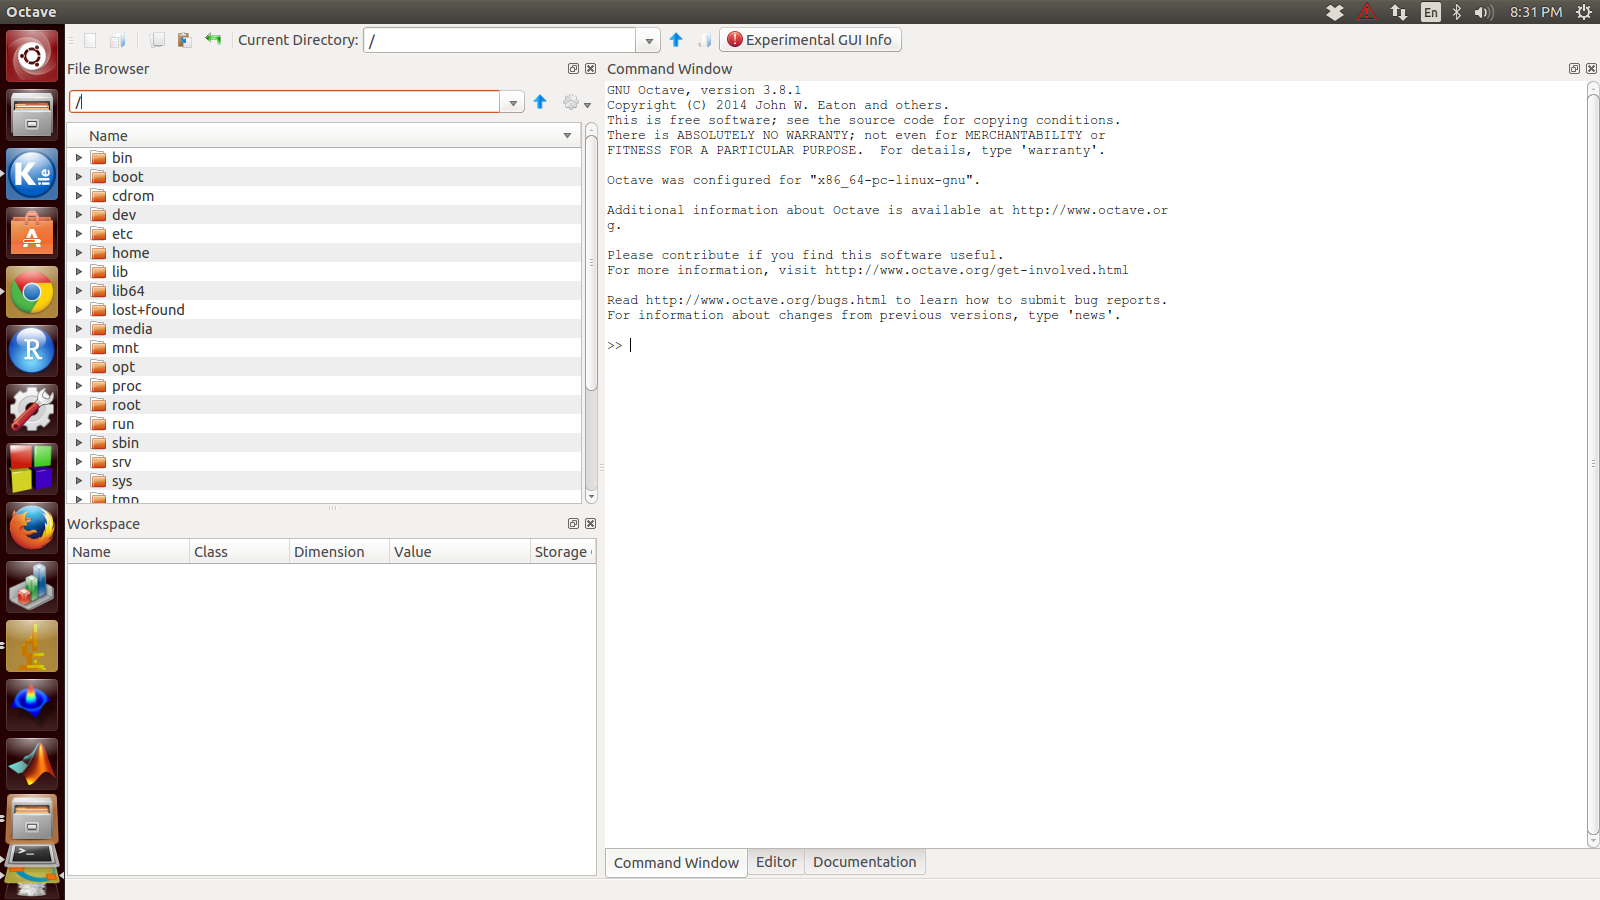
\includegraphics[scale=0.19]{images/OctaveGui.png} }
	\caption{Octave Graphical User Interface}
	\label{OctaveGui}
\end{figure}
\noindent It can also be used to write non-interactive programs. 
The Octave language is quite similar to Matlab so that most programs are easily portable.

\section{Conclusion}
This chapter covers existing system and problems they address, their limitation followed by proposed system to overcome the limitations.
The biological roots of CA, and also explanation of biological terminologies like CSC, TAC, TDC, ECM and proteolysis was covered.
Various softwares required for project like C++, Code::Blocks, GNU Octave, ImageJ, RStudio, MATLAB$\circledR$ ,QtiPlot and Apache OpenOffice were described.

